\section{BACKGROUND}\label{background}

In this section we provide an overview of the field of Reinforcement Learning and related work in designing algorithms to maximize an agent's reward in a given environment. We will then introduce the car racing simulation environment as well as past approaches to train agents to optimally navigate this environment.

\subsection{Reinforcement Learning}

The reinforcement learning task typically involves an agent interacting with an environment $\mathcal{E}$ having a state space $\mathcal{S}$ and action space $\mathcal{A}$ for a finite number of time steps where the agent can alter its behavior upon observing the consequences of its actions \cite{2.0}. At each time step $t$, the agent receives the current observable state $s_t \in \mathcal{S}$ from the environment and selects an action $a_t \in \mathcal{A}$ to take in state $s_t$. Upon receiving $a_t$, the environment then presents with agent with the next state $s_{t+1} \in \mathcal{S}$, a scalar value $r_t \in \mathbb{R}$ as feedback representing the reward or utility of taking action $a_t$ in state $s_t$. As an agent usually interacts with the environment in finite time intervals, the agent also receives a boolean flag $d_t$ representing whether the interaction has ended, usually due to reaching the time limit for each interaction, or from taking an action that lead to a terminal state. In this report, we will refer to the set of terms for each time step $(s_t, a_t, s_{t+1}, r_t, d_t)$ as an experience tuple, where a sequence of experience tuples from the initial time step to a terminal state is known as a rollout.

The goal of a reinforcement learning agent is to learn a mapping from states to actions in order to select the optimal actions based on the given input state such that the total reward over an entire rollout is maximized. This mapping is referred to as a policy $\pi(s) \rightarrow a \in \mathcal{A}$ where the next action to take is derived based on an input state. Such a policy is often learned by exploring the environment and tuning an initially random policy according to the reward signal observed from each action. Deep reinforcement learning involves representing a policy with a neural network and using gradient-based optimization algorithms to train it towards an optimal policy. Previous work in policy optimization has explored value-based approaches such as Deep Q-Learning, policy-based approaches such as neuroevolution, and hybrid approaches such as Actor-Critic algorithms.

\subsubsection{Deep Q-Learning}

Deep Q-Learning aims to model the expected value distribution of taking each action where the action with the highest expected value is selected. The value of taking a particular action is modeled using the optimal value function $Q^*(s,a)$ known as the Bellman equation and is defined in \cite{2.1.0} as:
\begin{dmath}
	Q^*(s_t,a_t) = \mathbb{E}_{s_{t+1} \sim \mathcal{E}} \left[ r_t + \gamma \max_a Q^*(s_{t+1},a) \right]
\end{dmath}
This approximates the expected discounted long-term reward (known as the Q-value) of taking action $a_t$ in state $s_t$ where $\gamma$ is the discount rate for future rewards and is typically between 0.9 and 0.99. Given this optimal value function, an optimal policy $\pi^*(s_t)$ will select the action with the maximum Q-value where $a_{t+1} = \pi^*(s_t) = \arg \max_a Q^*(s_t,a)$. The value function $Q(s,a)$ can be modeled using a neural network parameterized by $\theta$ denoted as $Q(s,a;\theta) \approx Q^*(s,a)$ and can be trained iteratively to minimize the following loss function $L_i(\theta_i)$ using stochastic gradient descent for the $i_{th}$ iterative update:
\begin{dmath}
	L_i(\theta_i) = \mathbb{E}_{s \sim \mathcal{E}, a \sim \pi(\cdot)} \left[ (y_i - Q(s,a;\theta_i))^2 \right], 
\end{dmath}
where $y_i = r + \gamma \max_a Q(s',a;\theta_{i-1})$ is the target value computed using the currently observed reward $r$ and next state $s'$. The Q-Learning algorithm is suited to environments with discrete actions and was able to achieve super-human performance on many Atari games where there are usually 4 possible actions \cite{2.1.1}. However, this approach is less effective for environments with continuous action spaces due to the policy's discretization of Q-values modeled for a certain number of actions. One solution is to discretize the continuous state space \cite{2.1.3}, however, this can lead to an exponential increase in the number of discrete actions \cite{2.2}.

\subsubsection{Policy Search}

Policy search algorithms are generally gradient-free approaches that aim to find the optimal policy by evaluating the performance of a population of agents with different network parameters, then perturbing the network parameters of the best-performing agents to generate the next population to evaluate. Unlike Deep Q-Learning, this approach learns a direct mapping from states to actions without relying on finding the maximum over the action-value space. These are known as evolutionary algorithms and are effective for smaller network architectures as fewer parameters leads to a smaller policy search space over possible combinations of parameter values \cite{2.0}. The Covariance Matrix Adaptation Evolutionary Strategy (CMA-ES) is an effective approach for modeling non-linear stochastic functions as it uses a multivariate Gaussian distribution for parameter sampling \cite{1.0.3}. It is popular for use in evolving neural network parameters as it is capable of searching solution spaces of up to a few thousand parameters \cite{1.0.0}. However, this places an implicit limit to the size and expressiveness of the neural network, where larger networks require larger population sizes in order to adequately explore the policy space.

\subsubsection{Actor-Critic Methods}

Actor-critic methods combine direct policy representation from policy search with gradient optimization enabled by value-based approaches. This consists of an ``actor'' network (policy) which is trained according to the feedback, also referred to as policy gradients, from a ``critic'' network (value function). Two popular actor-critic approaches explored in this paper are Deep Deterministic Policy Gradients (DDPG) \cite{2.2} and Proximal Policy Optimization (PPO) \cite{2.3}. 

For the DDPG algorithm, the critic network is trained to approximate the same optimal value function with the loss function from Deep Q-Networks where the target value is instead $y_i = r + \gamma Q(s',\pi(s';\phi_i);\theta_{i-1})$, where $\pi(s';\phi_i)$ is the direct policy of the actor network parameterized by $\phi$. The actor is trained simultaneously to maximize the value predicted by the critic of a selecting action $a_t$ taken in state $s_t$ according to the following loss function \cite{2.2}:

\begin{dmath}
	L_i(\phi_i) = -\mathbb{E}_{s \sim \mathcal{E}, a \sim \pi(s)} \left[ Q(s,\pi(s;\phi_{i-1});\theta_i) \right]
\end{dmath}

Recent improvements to the DDPG algorithm involve training the actor according to the predicted value of an action offset by a baseline value of the input state. This is known as the advantage and is calculated in \cite{2.1.2} as:
\begin{dmath}
	A(s,a) = Q(s,a) - \mathbb{E}_{a' \sim \pi(s)} \left[ Q(s,a') \right]
\end{dmath}
The actor can then be trained to maximize the advantage function according to a modified loss function:
\begin{dmath}
	L_i(\phi_i) = -\mathbb{E}_{s \sim \mathcal{E}, a,a' \sim \pi(s)} \left[ Q(s,\pi(s;\phi_{i-1});\theta_i) - Q(s,a';\theta_i) \right]
\end{dmath}

For PPO, the critic network uses the optimal action value function to model the baseline state value, $V(s;\theta)$, independent of action as where $y_i = r + \gamma V(s';\theta_{i-1})$. The actor network, $\pi(s;\phi) = \mathcal{N}(\mu(s;\phi),\sigma(\phi)^2)$, is a mapping from states to a probability distribution, over actions where the action $a_t \sim \pi(s_t;\phi_i)$ is sampled from this distribution, giving an associated probability of that action denoted $\pi_{\phi_i}(a_t|s_t)$. Then, the actor is trained to minimize the following loss function \cite{2.3}:
\begin{dmath}
	L_i(\phi_i) = \mathbb{E}_{t} \left[\min \left( p \hat{A}(s_t),\ \textrm{clip} \left(p, 1-\epsilon, 1+\epsilon \right) \hat{A}(s_t) \right) \right],
\end{dmath} 

where $p = \frac{\pi_{\phi_i}(a_t|s_t)}{\pi_{\phi_{i-1}}(a_t|s_t)}$ $\hat{A}(s_t) = r_t + \gamma V(s_{t+1}) - V(s_{t})$ is the advantage estimate. This loss function aims to adjust the probability of sampling actions from the next policy $\pi_{\phi_i}$ relative to the last policy $\pi_{\phi_{i-1}}$ based on the advantage of taking that action. The derivation of this loss function is available in \cite{2.3}.

\begin{figure}[ht!]
	\centering
	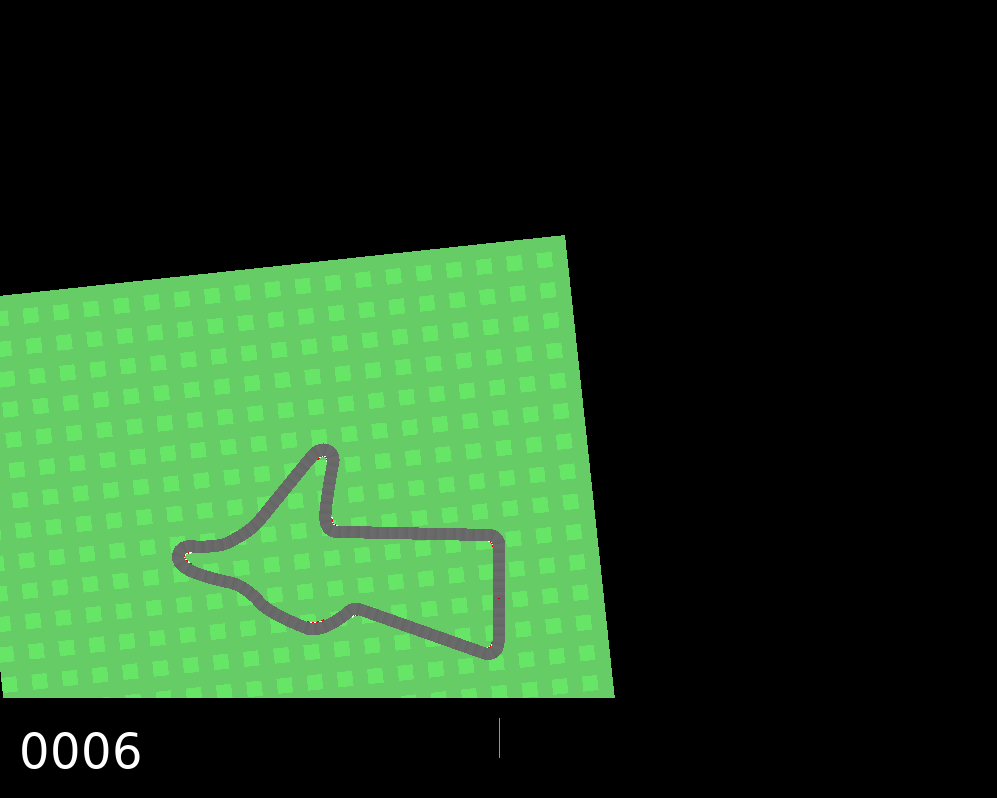
\includegraphics[width=0.45\textwidth]{images/car-map.png}
	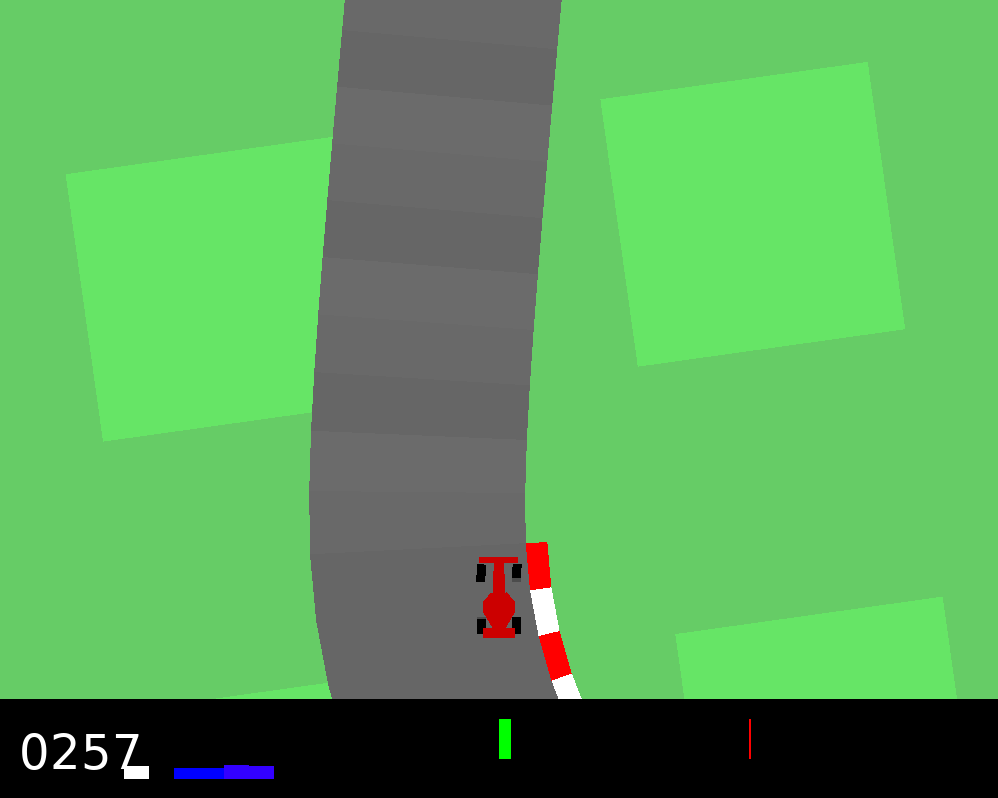
\includegraphics[width=0.45\textwidth]{images/car-tile.png}
	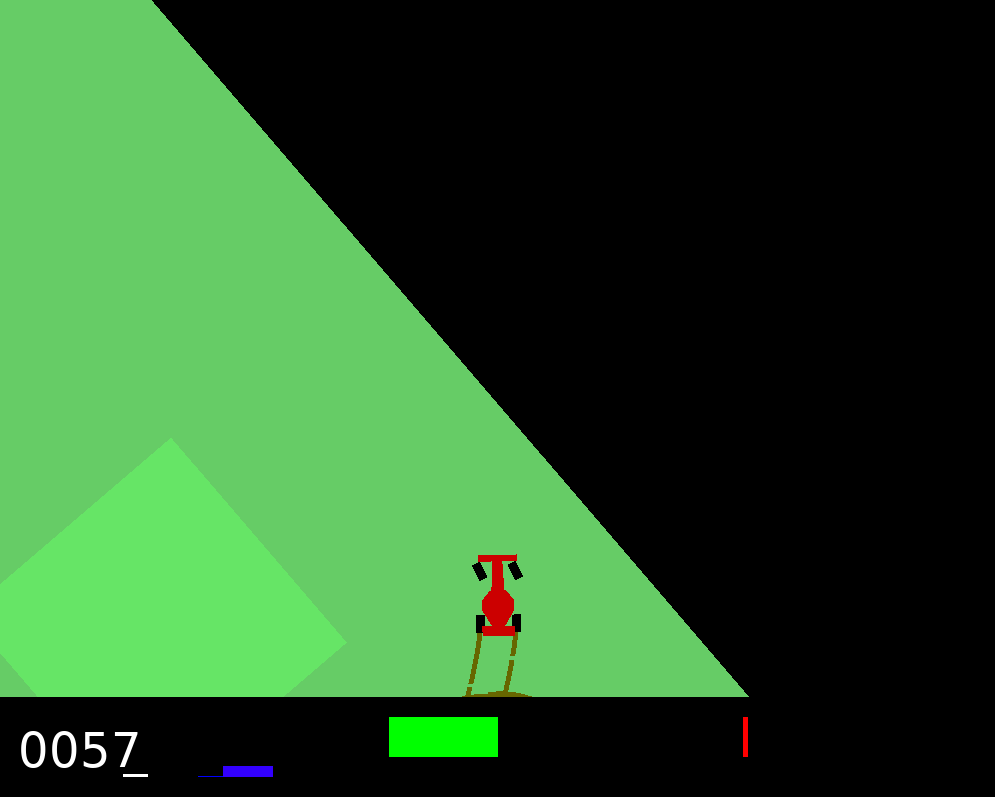
\includegraphics[width=0.45\textwidth]{images/car-die.png}
	\caption{Random Map (left), State Image (middle), Edge of map (right)}\label{fig:carracing}
\end{figure}

\subsection{OpenAI Gym's CarRacing-v0}

The \texttt{CarRacing-v0} environment is an open-source car racing simulator on the reinforcement learning platform OpenAI Gym \cite{0.0}. The goal is for an agent to control the steering, acceleration, and braking of the car to drive it along a randomly generated circuit track in as few time steps possible. At each time step $t$, the state $s_t$ is a 96x96 RGB image of the top view of the car on the map seen in Figure \ref{fig:carracing} in the middle. The agent then needs to provide an action consisting of three continuous values for the steering (between -1 and 1) and the acceleration and brake (between 0 and 1). The track is overlaid with $n$ (usually between 230 and 320) rectangular tiles (seen in the middle of Figure \ref{fig:carracing}) and the agent receives a reward of $1000/n$ upon visiting a tile for the first time. A rollout terminates after $1000$ time steps, if the agent visits every tile, or if it drives off the edge of the map (right of Figure \ref{fig:carracing}), in which case it receives a penalty (negative reward) of $-100$. The agent also receives a penalty or $-0.1$ at each time step, encouraging faster completion of the circuit. The environment is considered solved for an agent that achieves an average reward of at least $900$ over $100$ consecutive trials.

\subsection{Previous Approaches to Solve CarRacing-v0}

Recent work by Ha and Schmidhuber \cite{1.0.0} uses Variational Auto-Encoders (VAEs) to learn a compressed latent feature vector from the image states sampled from 10000 random rollouts. This simplified representation of states in the environment is then passed through a Gaussian Mixture Density Recurrent Neural Network (MDRNN) to model the temporal dynamics of the environment (known as the World Model) by predicting the next latent vector from a given action, the current latent vector, and the cumulative internal memory state. Finally, a simple feed-forward network is trained using the CMA Evolutionary Strategy to output an action given the latent representation and the internal memory of the MDRNN. This approach is the current state of the art for solving OpenAI Gym's \texttt{CarRacing-v0} environment achieving an average score of 906 over 100 trials. In the original paper \cite{1.0.0}, it was found that the state representation of the world model trained on random rollouts may not accurately represent the reward producing states of the environment. This can be improved with iterative training of the VAE and MDRNN with additional sequences of experience tuples sampled from rollouts using a trained world model agent.

Previous work in solving \texttt{CarRacing-v0} with Deep RL has also explored using Deep Q-Networks (DQN) and DDPG. Jang et al \cite{3.0} achieved a maximum score of 591 with a continuous asynchronous DDPG with edge detection preprocessing on input images. Gerber et al \cite{3.1} were able to achieve an average reward of 907 with a discretized DQN using the dropout regularization method. However, both of these approaches used manual discretization of the continuous action space to 5 discrete actions based on prior knowledge of operating a car which eliminates the original challenge of the task of independently selecting the steering, acceleration and braking from a continuous range. Therefore, this paper will focus on the effectiveness of the world model architecture to simplify the input states an agent receives in order to prioritize optimal continuous action selection without manual discretization or specialized image preprocessing.

% Both methods use a variation of the optimal value function from Deep Q-Networks to train the critic network, where in the case of DDPG, the actor is a deterministic mapping from states to actions trained to output actions that maximize the critic's predicted value of taking those actions in the given state. In the case of PPO, the actor is a mapping from states to a probability distribution over actions, trained to maximize the probability of selecting actions that lead to higher values than that of the previous iteration of the policy. The technical formulation of these two approaches will be detailed in Section \ref{tech:ddpg} and \ref{tech:ppo}.